\documentclass{article}
\usepackage[utf8]{inputenc}
\usepackage[utf8]{inputenc}
\usepackage{enumitem}
\setlist{nolistsep}
\usepackage[T1]{fontenc}
\usepackage[a4paper,left=1.5cm,right=1.5cm,top=2cm,bottom=2cm]{geometry}
\usepackage[frenchb]{babel}
\usepackage{libertine}
\usepackage[pdftex]{graphicx}
\usepackage{appendix}
\usepackage{multirow}
\usepackage{tipa}
\usepackage{float}
\usepackage{comment}
\usepackage[nottoc, notlof, notlot]{tocbibind}
\usepackage{hyperref}
\usepackage{geometry}
\usepackage[toc,page]{appendix} 
\geometry{hmargin=1.5cm,vmargin=1.5cm}
\setlength{\parindent}{0cm}
\setlength{\parskip}{1ex plus 0.5ex minus 0.2ex}
\newcommand{\hsp}{\hspace{20pt}}
\newcommand{\HRule}{\rule{\linewidth}{0.5mm}}
\renewcommand{\thesection}{\Roman{section}} 
\usepackage{caption}
\captionsetup[figure]{name=Fig.}
\title{Pédaler pour rappeler : l’effet du mouvement cyclique des mains et des jambes sur la narration d’histoires et la mémorisation de pseudo-mots}
\author{Alexandra Steinhilber\\ Amélie Rochet-Capellan et Marion Dohen \\ GIPSA-Lab, Grenoble Images Parole Signal Automatique \\ 10830 mots}
\date{Juin 2019}


\begin{document}


\section{Introduction}



\begin{comment}


\begin{resume} 
Abstract ..
\end{resume}

\cite{Burkhardt18}

\begin{itemize}[label=\textbullet, font=\small] %\LARGE
    \item D’un mini-vélo d'appartement 
    \end{itemize}

\begin{figure}[H]
\centering
	\includegraphics[scale=0.2]{Setup.png}
	\caption{Installation du participant}
	\label{Setup}
\end{figure} 

\begin{figure*}[!h]
\minipage{0.25\textwidth}
    \centering
	\includegraphics[scale=0.06]{dessin_detect.jpg}
	\caption{dessin au crayon}
    \centering
\endminipage
\minipage{0.25\textwidth}
	\includegraphics[scale=0.4]{dessin2_detect.jpg}
	\caption{dessin contour}
    \centering
\endminipage
\minipage{0.25\textwidth}
	\includegraphics[scale=0.4]{peinture_detect.jpg}
	\caption{peinture}
    \centering
\endminipage 
\minipage{0.25\textwidth}
	\includegraphics[scale=0.55]{dessin3_detect.jpg}
	\caption{dessins grossiers}
	\endminipage
\end{figure*}


\begin{table}[!ht]
    \small
    \center
    \begin{tabular}[b]{|l|c|c|c|}
    \hline
    A1 & A2 & A3 & A4 \\
    \hline \hline
    B1 & B2 & B3 & B4 \\
    %& \multicolumn{3}{|c|}{} \\
    \hline
    C1 & C2 & C3 & C4 \\
    \hline 
    \end{tabular}
    \caption{Variables de mémoire testées}
\end{table}

A LA FIN

\bibliographystyle{apalike}
\bibliography{Ref}

\appendix
\section{Annexe }\label{A}

\end{comment}

\section{Variables de cohérence}
Soient A et B 2 distributions définies sur le même espace, |A|=|B|=n

Distribution jointe : 
$$P(\la A B)=P(A)P(B)P(\la |AB)$$

\paragraph{Inférence classique}
\begin{align*}
P(\la =F) &=  \sum_{A,B}P(A)P(B)P(\la =F|AB) \\
 &= \sum_{A} P(A=a) \sum_{B=b\neq a} P(B=b)\\
 &=  \sum_{A}P(A=a) (1-P(B=a)) \\
 &= <P(A),1-P(B)> \\
 &= 1 -<P(A),P(B)> 
 \end{align*}
 
 \begin{align*}
P(\la =T) &=  \sum_{A,B}P(A)P(B)P(\la =T|AB) \\
 &= \sum_{A} P(A=a) P(B=a)\\
 &= <P(A),P(B)> \\
 \end{align*}
 
\begin{comment}
  \begin{align*}
P(\la =T) &=  \sum_{A,B}P(A)P(B)P(\la =T|AB) \\
 &= \sum_{A} P(A=a) P(B=a) P(\la=T|AB) +\sum_{A} \sum_{B=b\neq a}P(A=a) P(B=b) P(\la=T|AB) \\
  &= p1* \sum_{A} P(A=a) P(B=a) + (1-p2)* \sum_{A} \sum_{B=b\neq a}P(A=a) P(B=b)  \\
 &= p1 <P(A),P(B)> + (1-p2) <P(A),1-P(B)>\\
 &= (p1+p2-1) <P(A),P(B)> + (1-p2)\\
 \end{align*}
 
   \begin{align*}
P(\la =F) &=  \sum_{A,B}P(A)P(B)P(\la =F|AB) \\
 &= \sum_{A} P(A=a) P(B=a) P(\la=F|AB) +\sum_{A} \sum_{B=b\neq a}P(A=a) P(B=b) P(\la=F|AB) \\
  &= (1-p1)* \sum_{A} P(A=a) P(B=a) + p2* \sum_{A} \sum_{B=b\neq a}P(A=a) P(B=b)  \\
 &= (1-p1) <P(A),P(B)> + p2 <P(A),1-P(B)>\\
 &= -(p1+p2-1) <P(A),P(B)> + p2\\
 \end{align*}
 
    \begin{align*}
P(\la =F) &=  \sum_{A,B}P(A)P(B)P(\la =F|AB) \\
 &= \sum_{A} P(A=a) P(B=a) P(\la=F|AB) +\sum_{A} \sum_{B=b\neq a}P(A=a) P(B=b) P(\la=F|AB) \\
  &= p* \sum_{A} \sum_{B=b\neq a}P(A=a) P(B=b)  \\
 &=  p <P(A),1-P(B)>\\
 \end{align*}
 
 
\end{comment}


 Sémantique : 
 
 $P(\la=F)$ = probabilité de la présence d'une erreur = détection d'erreur (incohérence entre A et B)
 
 \paragraph{Inférence par négation moyenne}
 \begin{align*}
P(\la =F) &=\sum_{A,B}P(A)P(B)P(\la =F|AB) \\
 &=\sum_{A}P(A=a) P(\neg (B=a)) \\
 &=\sum_{A}P(A=a) \frac{1-P(B=a)}{n-1} \\
 &=<P(A),\frac{1-P(B)}{n-1}> \\
 &=\frac{1}{n-1} (1 -<P(A),P(B)>)
 \end{align*}
 
 Sémantique : 
 
 - on compare à une lettre moyenne "typique" et pas à toutes les autres ? 
 
 - on compare à une seule des n-1 lettres restantes (en considérant que la distribution est uniforme), et on regarde la similarité entre la lettre de la distribution A et cette lettre-là : on calculerait donc la proba d'avoir visé juste dans le tirage de cette unique lettre, ce serait plutôt une correction d'erreur qu'une détection ?  
 
 Mathématiquement, la distribution $\la$ ne somme plus à 1.
 
 \paragraph{Inférence par comparaison avec la meilleure alternative}
 

 \begin{align*}
P(\la =F) &=  \sum_{A,B}P(A)P(B)P(\la =F|AB) \\
 &= \sum_{A} P(A=a) \sum_{B=b\neq a} P(B=b)\\
 &=  \sum_{A}P(A=a) P(\neg (B=a)) \\
 &= \sum_{A} P(A=a) * \max_{B=b\neq a} (P(B=b))\\
 \end{align*}
 
On fait une approximation non linéaire après la ligne 2, peut être qu'elle pourrait être remplacé par l'introduction d'une nouvelle variable ? 
  
Sémantique : On compare avec la meilleure alternative possible : correction d'erreur réduite à 1 possibilité ?
  

  
  \section{Etude de l'opérateur de négation moyenne}

  Soit A une distribution définie sur $E=\{ a_1,...,a_n \}$, avec $\forall i \in \{ 1,..,n \}$, $P(A=a_i)=x_i$
  
  On définit l'opérateur négation associé à une distribution (car il dépend de son cardinal) par :\\
  $$P(\neg (A=a_i))=\frac{1-P(A=a_i)}{n-1}$$\\
  
  Après renormalisation, on peut ainsi définir une nouvelle distribution binaire $A_i$:\\
  $$P(A_i=a_i)=\frac{a_i*(n-1)}{1+(n-2)*a_i}$$\\
  $$P(\neg (A_i=a_i))=\frac{1-a_i}{1+(n-2)*a_i}$$ \\
  
  Sémantique : 
  
    - opérateur qui compare une possibilité aux autres en ne considérant pas la somme de toutes les possibilités, mais la moyenne.
    
  - permet de dire si une valeur est plus probable que les autres/comparaison relative aux autres valeurs de la distrib, pas à 1.
  
  - à 0.5, elle est "équivalente" aux autres valeurs, vers 0.9 elle sort largement du lot même si la pba en elle-même peut être faible.
  
  Propriétés :
  
  - Si on ne renormalise pas entre $A=a_i$ et $\neg(A=a_i)$, $\neg A$ est une distribution sur E.
  
  - Si l'on réapplique cet opérateur (avec la constante n) sur la distribution binaire :
  
    - ça ne donne évidemment pas la négation dans l'ensemble binaire car la taille de l'ensemble de définition de la distribution a changé :
      la constante associée à cet ensemble devient n=2
      
    - Néanmoins, si on applique l'opérateur associé à A et qu'on cherche à calculer la négation de la négation obtenue, on trouve : 

  
 \begin{align*}
 P(\neg \neg(A_i=a_i)) &\propto \frac{1-\frac{1-a_i}{1+(n-1)*a_i}}{n-1}\\
    &\propto \frac{a_i}{1+(n-2)*a_i}
 \end{align*}
  Si on renormalise dans l'espace binaire entre $P(\neg \neg(A'=a_i))$ et $P(\neg (A'=a_i))$, on obtient :
  $$P(\neg \neg(A_i'=a_i)) = a_i$$ -> le nom $A_i$ ne correspond pas vu qu'on a utilisé l'opérateur 26 dans l'espace binaire non ?
  $$P(\neg(A_i'=a_i)) = 1-a_i$$

  Cette opération nous permet donc de renverser le processus et définir une bijection entre l'ensemble $\{x_1,..x_n\}$ associé à la distribution de probabilité A et n couples $\{y_i,\neg y_i\}$ associés à des lois $A_i$.

 \paragraph{Simu avec Python }
  On tire à l'infini selon la loi de proba discrète $P(A_i=ai)$ VS uniforme pour les nombres restants. ex [0.2]+[0.04]*20. On choisit une autre lettre à laquelle s'intéresser, par exemple la lettre 2. On compte le nombre de 0 et de 2, on normalise à la fin du tirage. 
  
  Résultat : on tombe sur la proba de la négation moyenne. 
  Le résultat sera évidemment pareil si on s'intéresse à 1 autre lettre car on considère la reste de l'espace distribué uniformément.
  La négation moyenne semble donc représenter la proportion entre le nombre de A tirés et une autre lettre (précise) parmi l'uniforme restante.

  
\paragraph{Interprétation}
    Est-ce qu'on peut interpréter ça comme la comparaison à une lettre "typique" plutôt qu'à une lettre précise parmi les n-1 restantes ?
    
  Si la distribution est uniforme on a assez d'information pour conclure que cette lettre là "sort du lot" (en même temps dans ce cas là 0.1 donne toute l'info existante, suffit pour définir précisément la distribution), donc on peut bien interpréter comme une comparaison de cette lettre aux autres.
  
  Mais si une autre lettre sort du lot, par l'hypothèse d'uniformité elle sera noyée dans le reste de la masse, et donc on n'a pas assez d'information pour conclure que 0.1 est la meilleure option. 
  
  Par exemple dans Braid si on a Pa=0.3 et Pe=0.6, $Pautre\simeq 0$ -> opérateur neg sur Pa = 0.91 VS 0.09, opérateur neg sur Pe = 0.97 VS 0.03
  -> $\neg Pa$ ne représente pas vraiment la situation où "ce n'est pas a" (négation). 
  -> Cet opérateur permet de savoir si une lettre "sort du lot", pas si elle est la plus probable \\
  -> dans Braid c'est plutôt la lettre VS UNE alternative, la correction (0.3 0.6 vs broutilles) (idée de prendre la meilleure alternative)\\


  
 \section{Propositions dans Braid}
  
  - l'opérateur de négation moyenne a-t-il la bonne sémantique ?
  
  - si on le laisse, l'erreur détectée est écrasée et les pseudo-mots ne sont pas détectés comme tels.
  
  - si on l'enlève, la détection d'erreur est trop importante : la détection initiale (perception uniforme) aboutit tout de suite à une DL=0 $\rarr$  comportement instable qui donne par exemple : help DL=0.9 à la fin, finit jamais à 0.99.

  EDIT\\
- on peut faire évoluer la pénalisation de la détection d'erreur en fonction du temps, plus précisément en fonction de l'état des connaissances : lorsqu'on n'a pas encore beaucoup d'informations, ce n'est pas la peine de comparer les connaissances orthographiques avec la perception des lettres, donc on ne détecte que très peu l'erreur. 

Lorsqu'on commence à accumuler des évidences perceptives, on devient un peu plus certain d'avoir véritablement détecté une erreur, on peut donc diminuer le coefficient de pénalisation.
Une idée est de diviser au sein de chaque comparaison (produit scalaire), par la norme 2 de la distribution des P. Cela revient à remplacer le produit scalaire du calcul par une information basée uniquement sur les angles entre les distributions (le cosinus).

Au début, lorsqu'on est proche de l'uniforme, cela revient à pénaliser l'erreur à une position quelconque en la multipliant par $\frac{1}{|P|-1}$, et ce coefficient augmente au fur et à mesure de l'accumulation d'évidences perceptives. On détecte donc de mieux en mieux l'erreur.

  

  \subsection{Comparaison de L et P dans Braid en divisant par la norme}
  
  Soient N la longueur du stimulus et k la taille de l'alphabet.
  
  Pour appliquer cette idée dans Braid, la portion de calcul contenant :
 $$ \prod_{i=1}^{N} <P(L_i|w^T),QP_i^T> $$ est remplacée par :
 $$ \prod_{i=1}^{N} <\frac{P(L_i|w^T)}{||P(L_i|w^T)||},\frac{QP_i^T}{||QP_i^T||}>$$
 
 Pour la simplicité des calculs, on enlèvera la norme de P(L) des calculs, valant environ 1 de toute manière (quasi-Dirac)
 
 On déroule les calculs lorsque DL=Yes:
  $$ \prod_{i=1}^{N} <P(L_i|w^T),\frac{QP_i^T}{||QP_i^T||}> = \frac{1}{\prod_{i=1}^{N} ||QP_i^T||} * \prod_{i=1}^{N} <P(L_i|w^T),QP_i^T> $$
  
  Et lorsque DL=No avec une erreur en position j :
\begin{eqnarray}
\lefteqn{\prod_{i=1,i \neq j}^{N} <P(L_i|w^T),\frac{QP_i^T}{||QP_i^T||}> * <P(L_j|w^T),\frac{1-QP_j^T}{||1-QP_j^T||}> }\\
& = &\frac{1}{\prod_{i=1}^{N} ||QP_i^T||}*\frac{||QP_j^T|| }{||1-QP_j^T||} * \prod_{i=1,i \neq j}^{N} <P(L_i|w^T),QP_i^T>* <P(L_j|w^T),1-QP_j^T>
\end{eqnarray}
     
     Le coefficient $\frac{1}{\prod_{i=1}^{N} ||QP_i^T||}$ apparaît indépendamment de la position de l'erreur et même de l'existence ou non d'une erreur (on le trouve dans DL=Yes et DL=No), il disparaîtra donc à la normalisation et peut être omis.
     
     Par rapport au calcul de DL effectué jusqu'à maintenant, il n'y a donc aucun changement dans le cas DL=Yes et une multiplication par un facteur $\frac{||QP_j^T|| }{||1-QP_j^T||}$ pour une erreur en position j.
     
     En Résumé : diviser par la norme au moment du produit scalaire revient à multiplier le calcul final de la probabilité d'avoir une erreur en position j par un coefficient $r_j=\frac{||QP_j^T|| }{||1-QP_j^T||}$, rapport entre 2 normes, .
     
     
     
    Si $P_j$ prend les valeurs $\{P_{j1}...P_{jk}\}$ avec des probabilités respectivement égales à $\{p_1...,p_k\}$, on a :
    $\forall j, \frac{||1-QP_j^T||^2}{||QP_j^T||^2}=\frac{\sum_{l=1}^{k}(1-p_l)^2}{\sum_{l=1}^{k}p_l^2}=1+\frac{k-2}{||QP_j^T||^2}$
    
    A l'initialisation (distribution uniforme), $$||QP_j^T||^2=\sum \frac{1}{k^2} = \frac{1}{k}$$
    
    donc $$\frac{||1-QP_j^T||^2}{||QP_j^T||^2}=1+k(k-2)=(k-1)^2$$
    
    et finalement
    $$\frac{||QP_j^T||}{||1-QP_j^T||}=\frac{1}{k-1}$$
    
    Initialement, la pénalisation vaut donc $\frac{1}{k-1}$, ce qui correspond à la version de la négation moyenne (faire les moyenne des k-1 alternatives).
    On a donc la bonne sensibilité au début, mais la dépénalisation progressive permet de tout de même détecter les pseudo-mots comme tels.
    
    
    \subsection{Comparaison de L et P dans Braid en divisant par la norme, cas où l'on détecte 2 erreurs!}
  
Rien ne change lorsque la DL vaut 1, on a le même produit qui apparaît et qu'on voudrait faire apparaître lorsque DL=0 pour pouvoir renormaliser et simplifier le calcul.
  
  Et lorsque DL=No avec une erreur en position j, et une en position l :
\begin{eqnarray}
\lefteqn{\prod_{i=1,i \neq j,l}^{N} <P(L_i|w^T),\frac{QP_i^T}{||QP_i^T||}> * <P(L_j|w^T),\frac{1-QP_j^T}{||1-QP_j^T||}> * <P(L_l|w^T),\frac{1-QP_l^T}{||1-QP_l^T||}> }\\
& = &\frac{1}{\prod_{i=1}^{N} ||QP_i^T||}*\frac{||QP_l^T|| }{||1-QP_l^T||} * \frac{||QP_j^T|| }{||1-QP_j^T||} * \prod_{i=1,i \neq j,l}^{N} <P(L_i|w^T),QP_i^T>* <P(L_j),1-QP_j^T> <P(L_l),1-QP_l^T>
\end{eqnarray}
     
     Le coefficient $\frac{1}{\prod_{i=1}^{N} ||QP_i^T||}$ apparaît indépendamment de la position de l'erreur et même de l'existence ou non d'une erreur (on le trouve dans DL=Yes et DL=No), il disparaîtra donc à la normalisation et peut être omis.
     
     Par rapport au calcul de DL effectué jusqu'à maintenant, il n'y a donc aucun changement dans le cas DL=Yes et une multiplication par 2 facteurs $r_{Pj}r_{Lj}$ et $r_{Pl}r_{Ll}$.
     
     En Résumé : diviser par la norme au moment du produit scalaire revient à multiplier le calcul final de la probabilité d'avoir 2 erreurs en position j et l par un coefficient $r_j*r_l=\frac{||QP_j^T|| }{||1-QP_j^T||}*\frac{||QP_l^T|| }{||1-QP_l^T||}$, rapport entre 2 normes, .
     
     
    En reprenant les mêmes notations que précédemment, à l'initialisation (distribution uniforme), 
    $$\frac{||QP_j^T||}{||1-QP_j^T||}=\frac{1}{k-1}$$
    et donc 
    $$\frac{||QP_j^T||}{||1-QP_j^T||}\frac{||QP_l^T||}{||1-QP_l^T||}=\frac{1}{(k-1)^2}$$
    Initialement, la pénalisation vaut donc $\frac{1}{(k-1)^2}$, ce qui correspond à la version de la négation moyenne si l'on détecte plusieurs erreurs.
    On a donc la bonne sensibilité au début, mais la dépénalisation progressive permet de tout de même détecter les pseudo-mots comme tels.
    
    En fixant 2 $\la$ à 0 si l'on veut détecter 2 erreurs, on pourra bien faire apparaître ce double produit.
    

    
    \subsection{Modification du modèle pour faire apparaître une division par la norme}
    
    L'idée derrière cette atténuation de la détection de l'erreur en divisant par la norme 2 de de P(P) est de pénaliser la détection d'erreur sans pour autant affecter la détection de correspondance ($\la=1$). En effet, dans une définition classique des variables de cohérence, il y a soit correspondance, soit non-correspondance. Chaque erreur non détectée se traduit donc par une détection de correspondance, ce qu'on cherche à éviter.
    
    Une idée pourrait donc être de définir une variable de cohérence ternaire : soit on détecte une correspondance, soit on détecte un mismatch, soit on ne détecte rien (état poubelle).
    
    En ramenant à 2 variables A et B que l'on chercherait à comparer et dont on connaît les coefficients $r_A$ et $r_B$ correspondant à $\frac{||A||}{||1-A||}$ et $\frac{||B||}{||1-B||}$ , on peut définir lorsque A=B:
    $$ P(\la = 0 |A=B)=0$$
    $$ P(\la = 1 |A=B)=1$$
    $$ P(\la = 2 |A=B)=0 $$
    Et lorsque A $\neq$ B : 
    $$ P(\la = 0 |A\neq B)=r_Ar_B$$
    $$ P(\la = 1 |A\neq B)=0$$
    $$ P(\la = 2 |A\neq B)=1-r_Ar_B$$
    
    Ainsi, on a :\\
\begin{align*}
P(\la =0) &=  \sum_{A,B}P(A)P(B)P(\la =0|AB) \\
  &= r_Ar_B \sum_{A}P(A=a) (1-P(B=a))\\
 &= r_Ar_B<P(A),1-P(B)> \\
 \end{align*}
 
\begin{align*}
P(\la =1) &=  \sum_{A,B}P(A)P(B)P(\la =1|AB) \\
  &= \sum_{A}P(A=a) P(B=a)\\
 &=<P(A),P(B)> \\
 \end{align*}
 
\begin{align*}
P(\la =2) &=  \sum_{A,B}P(A)P(B)P(\la =2|AB) \\
  &=(1-r_Ar_B)* \sum_{A}P(A=a)(1-P(B=a))\\
 &=(1-r_Ar_B)* <P(A),1-P(B)> \\
 \end{align*}
 
 
\subsection{Application du calcul dans Braid}
    
Voici un schéma simplifié des relations de dépendance imaginées dans Braid : 
\begin{figure}[H]
\centering
	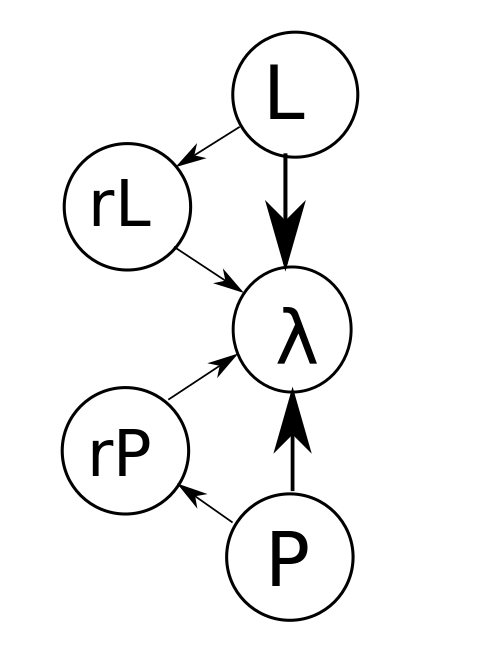
\includegraphics[scale=0.2]{dessin.png}
	\caption{Dessin simplifié}
	\label{Setup}
\end{figure} 

Les distributions $r_P$ et $r_L$ sont des Dirac dont le pic se situe au niveau de $\frac{||P||}{[[1-P||}$ et $\frac{||L||}{[[1-L||}$ respectivement.\\
TODO comment écrire ça ? Comme les définitions sont locales en général, du style $P(r_p=i|P=p_i)$



Pour le calcul de similarité, on va continuer, comme dans l'ancienne version, à imposer $\la=0$ pour une détection d'erreur et $\la=1$ pour une correspondance. On ne fixera donc jamais $\la$ à 2, et l'information "poubelle" ne sera jamais utilisée.

Le calcul de la DL est identique mis à part le fait que, lorsque $\la=0$, il fait apparaître ce coefficient $r_Pr_L$ équivalent à une division par la norme au moment du produit scalaire. Comme on ne considère que le cas où il y a une seule erreur, on n'imposera toujours qu'une seule fois $\la=0$, et le coefficient $r_Pr_L$ ne sera qu'une seule fois en facteur.

TODO latex de thierry pour éviter de recopier tous les calculs intermédiaires de la DL ?
 
 
  

    
\subsection{Simulations d'une version simplifiée de la DL}

On peut simuler une progression simplifiée de DL pour un dictionnaire ne contenant qu'un seul mot de 3 lettres, abc, avec un alphabet de 26 lettres. On décide de la progression des variables P et il n'y a pas d'attention mise en jeu.

\paragraph{mot correct : abc}
Les variables P convergent vers a,b,c en suivant une sigmoïde classique dans Braid.


\begin{figure}[H]
\centering
	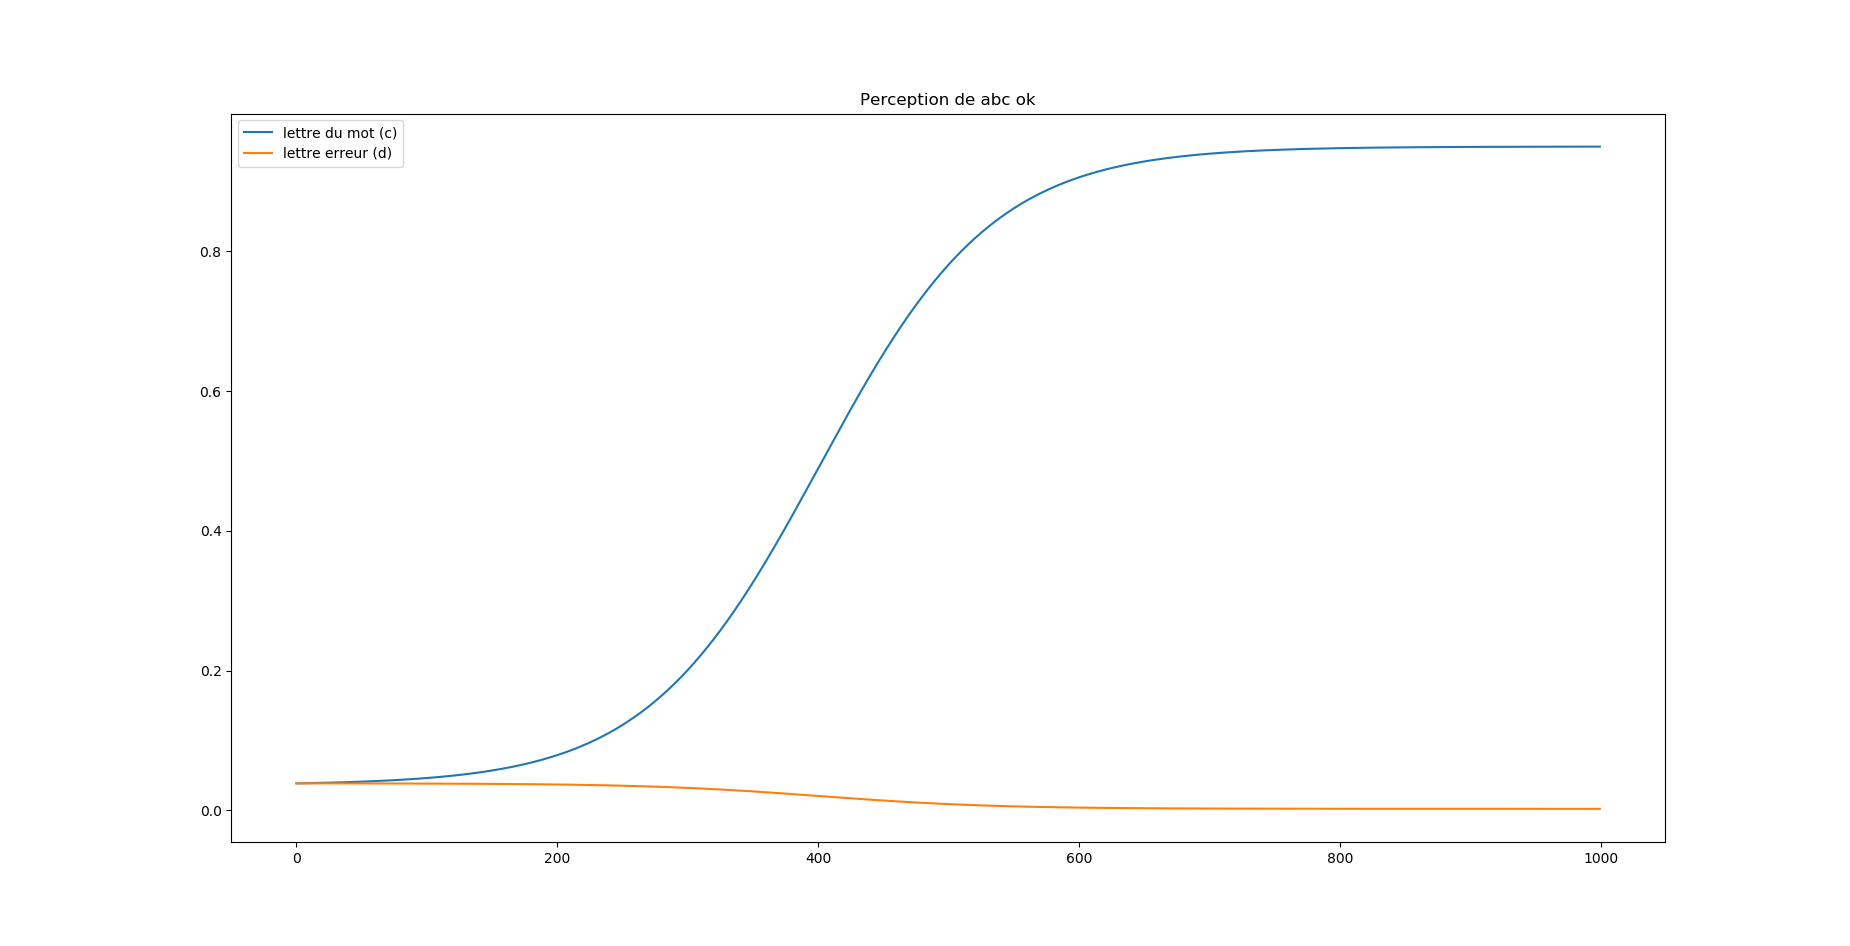
\includegraphics[scale=0.3]{P_abc.png}
	\caption{évolution des P décidée (pas calculée)}
\end{figure} 


Voilà le résultat de la simulation lorsque le mot abc, seul mot du dictionnaire, est présenté.

\begin{figure}[H]
\centering
	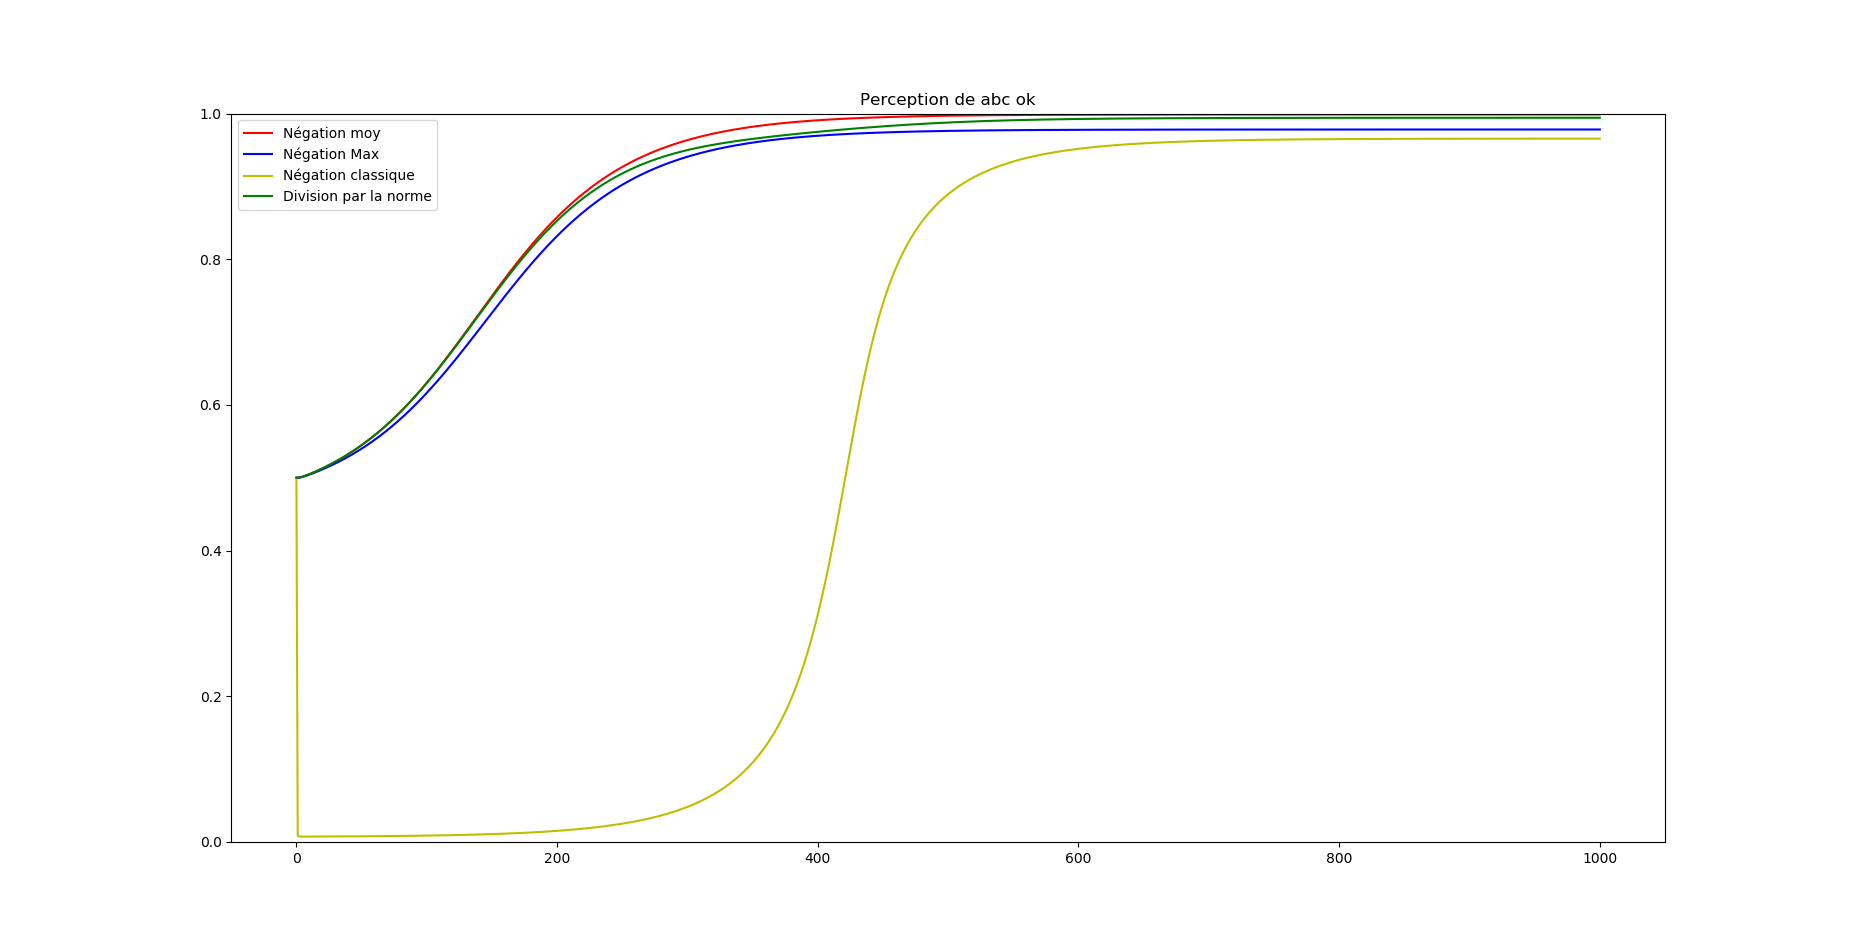
\includegraphics[scale=0.3]{abc.png}
	\caption{DL=Yes en fonction du type de simulation}
\end{figure} 


On voit que les 3 versions (négation moyenne, négation max, division par la norme) donnent des résultats assez similaires. La négation classique donne un comportement instable.
    
\paragraph{erreur : mot abd}
On a pour P une sigmoïde similaire mais convergeant vers la mauvaise lettre.
Voilà le résultat de la simulation lorsque le mot abd, pas dans le dictionnaire (composé uniquement de abc), est présenté.

\begin{figure}[H]
\centering
	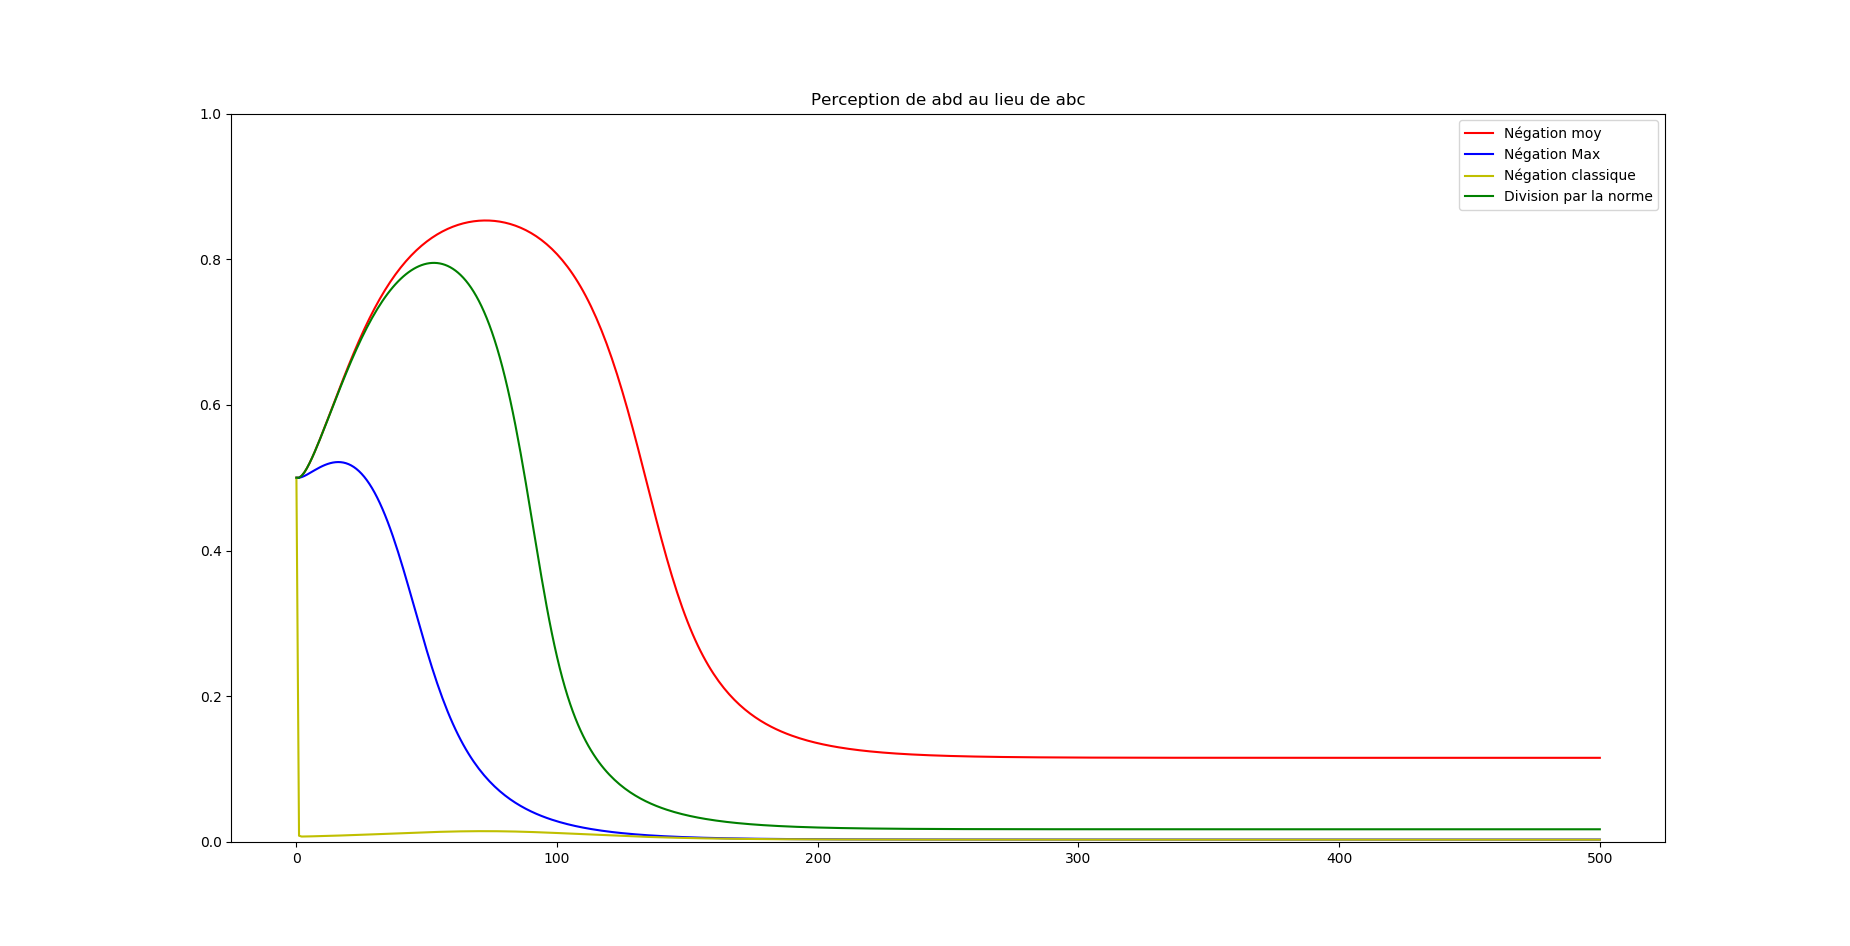
\includegraphics[scale=0.3]{abd.png}
	\caption{DL=Yes pour le mot abd (erreur)}
\end{figure} 

On voit que la négation max est plus rapide que la division par la norme pour s'orienter vers un non, même si les 2 versions semblent similaires à convergence. 

La version négation moyenne met plus longtemps à s'orienter vers un non et son asymptote n'est pas aussi basse que les 2 autres simulations : sûrement un défaut pour détecter les pseudo-mots dû à un défaut de comparaison.

Il y a quand même une envolée vers oui qui dure assez longtemps pour la version "division par la norme" 

TODO (et n'est pas satisfaisante ?). 

Elle est probablement dûe au fait qu'il y a un seul mot dans le dictionnaire et que les 2 mots (celui du dictionnaire et celui testé) sont voisins. Dans un dictionnaire plein, la comparaison au bon mot est "diluée" par la présence des autres mots (par l'intermédiaire de P(W0)). Si on fait tourner Braid avec un seul mot dans le dictionnaire, on retrouve ce genre de comportement. 

\paragraph{erreur : mot add (non voisin)}

\begin{figure}[H]
\centering
	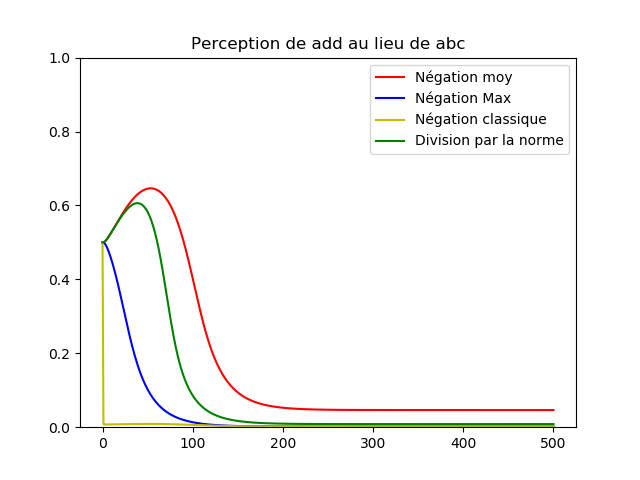
\includegraphics[scale=0.5]{add.png}
	\caption{DL=Yes pour le mot abd (erreur)}
\end{figure} 


pour un mot non voisin comme add, on voit que le pic est beaucoup moins marqué.
On remarque encore la différence d'asymptote entre les version "négation moyenne" et "division par la norme", ce qui est logique puisqu'on a un coefficient de pénalisation de l'erreur différent entre les 2 versions, plus particulièrement à la fin.



    
\paragraph{2 pics dans P, mot correct au niveau du plus grand pic}
On a pour P 2 sigmoïdes : 
la plus grande converge vers la bonne lettre et la plus petite vers la mauvaise lettre.

\begin{figure}[H]
\centering
	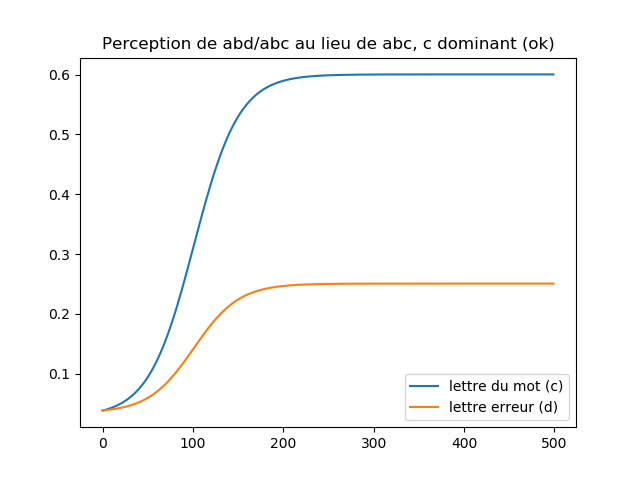
\includegraphics[scale=0.6]{P_abC_abd.png}
	\caption{évolution des P avec 2 pics}
\end{figure} 

Voilà le résultat pour la DL :

\begin{figure}[H]
\centering
	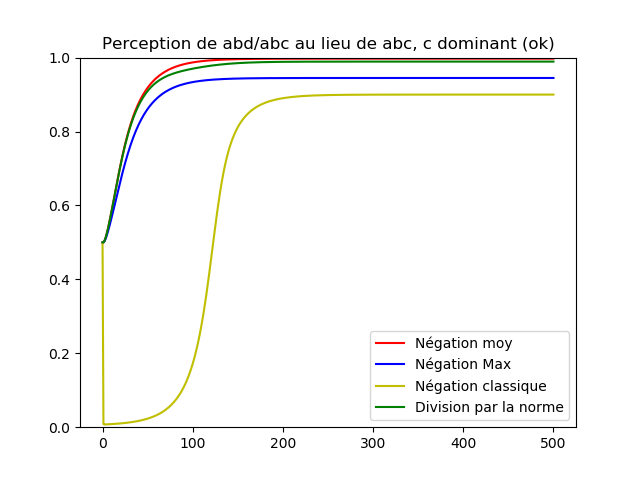
\includegraphics[scale=0.6]{abC_abd.png}
	\caption{DL=Yes pour le mot abC-abd (mot correct)}
\end{figure} 


L'objectif ici est de détecter le mot comme correct.

La version "division par la norme" atteint la même asymptote que la version négation moyenne, alors que la négation max atteint une asymptote légèrement plus faible.
TODO On obtient parfois ce cas dans Braid, quelle est le comportement cherché par rapport à l'humain ??
    
\paragraph{2 pics dans P, erreur au niveau du plus grand pic}
On a pour P 2 sigmoïdes : la plus grande converge vers la mauvaise lettre et la plus petite vers la bonne lettre. On voudrait donc détecter une erreur.

Voilà le résultat pour la DL :

\begin{figure}[H]
\centering
	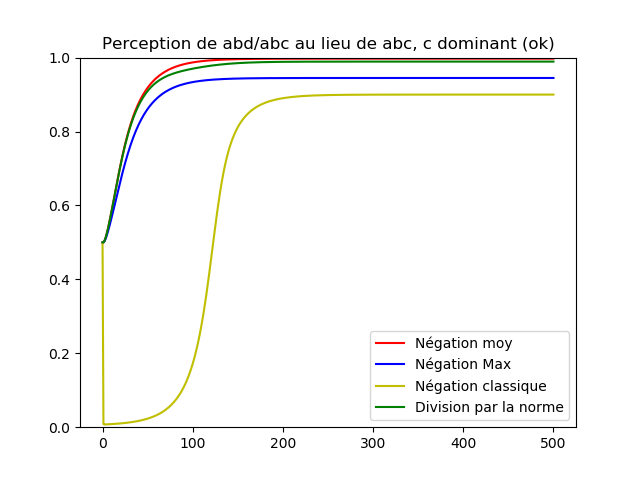
\includegraphics[scale=0.6]{abC_abd.png}
	\caption{DL=Yes pour le mot abc-abD (mot incorrect)}
\end{figure} 

La négation max reste dans l'incertitude, ce qui correspond bien à l'idée des deux courbes croissantes dans P, mais la version "division par la norme" rejoint presque l'asymptote à 1, l'erreur n'est pas détectée malgré une alternative prometteuse.

On peut expliquer ça par le fait que la comparaison compare intrinsèquement une valeur et l'ensemble des alternatives, mais pas une alternative (comme la version négation max). Il n'est pas donc pas possible de savoir s'il existe une meilleure alternative à celle-ci.
TODO : Peut être que c'est ce qu'on veut finalement ?

\begin{figure}[H]
\centering
	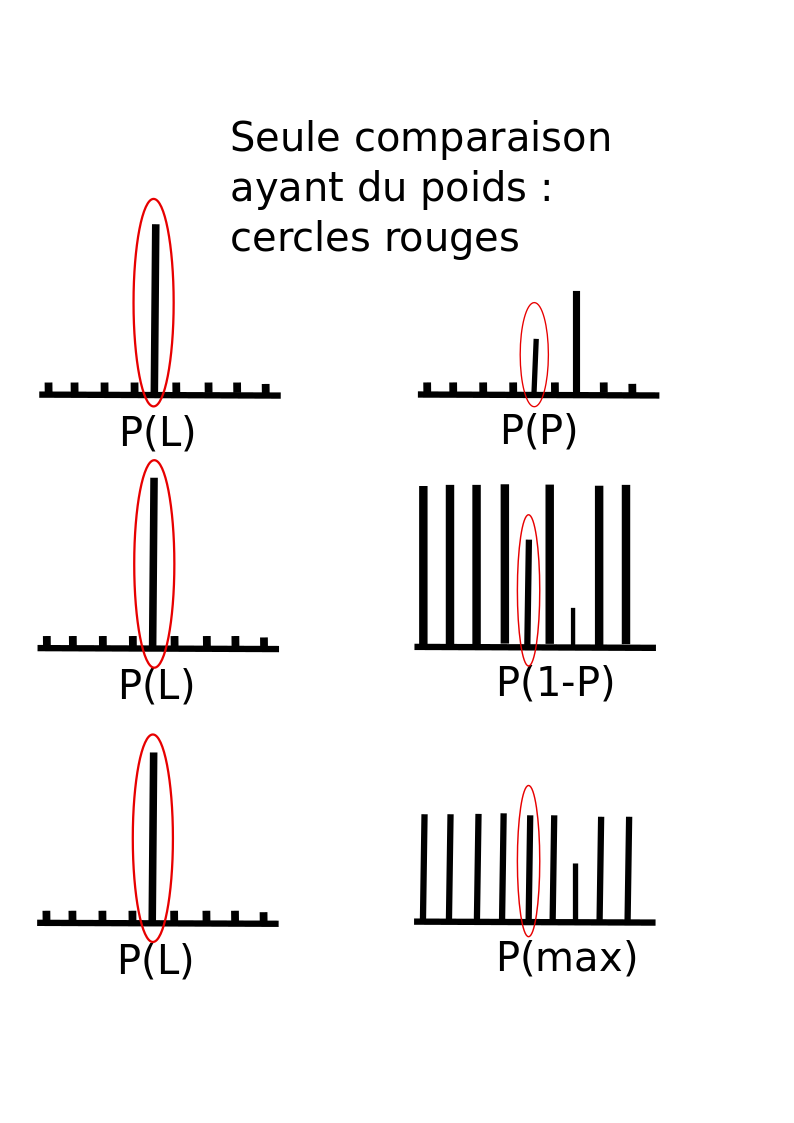
\includegraphics[scale=0.3]{schemaPL.png}
	\caption{schéma explicatif de la comparaison faite}
\end{figure} 
 
    
Ce schéma explicatif montre la comparaison faite selon la version de Braid lorsqu'on a 2 pics, dont 1 plus important.

- Première ligne : la seule comparaison qui a du poids est la multiplication entre les 2 barres rouges. Les autres barres de droite seront multipliées par un nombre très petit (barres de gauche), l'epsilon du quasi-Dirach. Cela ne ferait donc aucune différence d'avoir une uniforme sur toutes les autres barres que la barre entourée.

Ainsi, on ne se rend pas compte qu'il y a une meilleure alternative.

- Deuxième ligne : losqu'on calcule la négation, encore une fois seule la valeur du pic rouge importe, pas l=celle des alternatives.

- Dernière ligne : La comparaison importante concerne la meilleure des alternatives dans le cas de la négation max, on se rend donc compte qu'il y a une meilleure alternative même si la proposition courante n'est pas si mal.

TODO : est-ce qu'on a imaginé ce cas-là parce qu'on a approfondi la négation max et l'idée de la meilleure des alternatives, et donc est-ce que la présence de 2 courbes croissantes dans P est tellement peu fréquente que pas intéressante à étudier ?
On a sûrement mieux à simuler ? 
    
\paragraph{Bilan}

Pour un mot correct, l'asymptote était plus basse avec la version "négation max", et la version "division par la norme" atteint la même asymptote que la version "négation moyenne". Le résultat est donc satisfaisant.

Pour un mot incorrect, c'est l'inverse : l'asymptote atteinte par la version "négation moyenne" est beaucoup trop haute, et la version "division par la norme" se rapproche beaucoup plus de l'asymptote de la version "négation max", qui est beaucoup plus satisfaisante.

Pour résumer, la version "division par la norme" semble plus adaptative en convenant aussi bien aux cas des erreurs et des vrais mots à la fois.

\section{Aparté modification de la formule pour optimiser le calcul}
 
 On déroule les calculs lorsque DL=Yes:
  $$ \prod_{i=1}^{N} <P(L_i|w^T),\frac{QP_i^T}{||QP_i^T||}> = \frac{1}{\prod_{i=1}^{N} ||QP_i^T||} * \prod_{i=1}^{N} <P(L_i|w^T),QP_i^T> $$
  

lorsque DL=No avec une erreur en position j :
\begin{eqnarray}
\lefteqn{\prod_{i=1,i \neq j}^{N} <P(L_i|w^T),\frac{QP_i^T}{||QP_i^T||}> * <P(L_j|w^T),\frac{1-QP_j^T}{||1-QP_j^T||}> }\\
& = &\frac{1}{\prod_{i=1}^{N} ||QP_i^T||}*\frac{||QP_j^T|| }{||1-QP_j^T||} * \prod_{i=1,i \neq j}^{N} <P(L_i|w^T),QP_i^T>* <P(L_j|w^T),1-QP_j^T>
\end{eqnarray}

Le facteur $\frac{1}{\prod_{i=1}^{N} ||QP_i^T||}$ est présent pour Yes et No, on peut donc l'enlever (propto).

Le calcul (dans le code) consiste à stocker dans un tableau [DL=Yes,Erreur0,Erreur1], soit :
$(1,\frac{||QP_0^T||}{||1-QP_0^T||},\frac{||QP_1^T||}{||1-QP_1^T||}..)$

  Si $P_j$ prend les valeurs $\{P_{j1}...P_{jk}\}$ avec des probabilités respectivement égales à $\{p_1...,p_k\}$, on a :
    $\forall j, \frac{||1-QP_j^T||^2}{||QP_j^T||^2}=\frac{\sum_{l=1}^{k}(1-p_l)^2}{\sum_{l=1}^{k}p_l^2}=1+\frac{k-2}{||QP_j^T||^2}$
    
Donc $\frac{||QP_j^T||}{||1-QP_j^T||}=\sqrt{\frac{1}{1+\frac{k-2}{||QP_j^T||^2}}}=\frac{1}{\sqrt{1+\frac{k-2}{||QP_j^T||^2}}}$

 
 $P(L_n^{1} | W^{1} = w) \propto U \times P(P_{n}^{1} | S_{n}^{1}) \propto P(P_{n}^{1} | S_{n}^{1})$
 
 $P(L_n^{f+1} | W^{f+1} = w) \propto P(L_n^f | W^f=w) \times ((1-\alpha)\times U + \alpha \times P(P_{n}^{1} | S_{n}^{1}))$
 
 with $ \alpha = \frac{1}{f+1}$
 
 

 
\end{document}

